\section*{Introduzione}
Appunti di geometria e algebra lineare di Nadif Nizar, studente di scienze dell'informazione presso l'università degli studi di Trento.
Questi appunti sono stati presi nel primo semestre dell'anno scolastico 2021/2022, seguendo i corsi del prof. Alessandro Perotti.

\chapter{Gruppi}

Dati i seguenti insiemi:
$$ \mathbb{N} \subset \mathbb{Z} \subset \mathbb{Q} \subset \mathbb{R} \subset \mathbb{C} $$

Ricordiamo alcune delle seguenti operazioni:
\begin{itemize}
	\item $ x = a + b $ non sempre ha soluzioni in $ \mathbb{N} $;
	\item $a \cdot x = b $ non sempre ha soluzioni in $ \mathbb{N} $ e $ \mathbb{Z} $;
	\item $ x^2 = 2 $ non ha soluzioni in $ \mathbb{N}, \mathbb{Z}, \mathbb{Q} $;
\end{itemize}

Infine i numeri complessi, il cui insieme è denotato con $ \mathbb{C} $, permettono di risolvere tutte le equazioni polinomiali.


\section{Definizione}
	Un gruppo è un insieme  $ \mathbb{G} $ su cui è definita un'operazione $ * $ con le seguenti proprietà:
	\begin{enumerate}
		\item associativa: $ ( a * b ) * c = a * ( b * c) \quad \forall a, b, c \in \mathbb{G} $;
		\item esistenza dell'elemento neutro: $ \exists e \in \mathbb{G} | a * e = e * a = a \quad \forall a \in \mathbb{G} $;
		\item esistenza dell'elemento simmetrico: $ \forall a \in \mathbb{G} \quad \exists a' \in \mathbb{G} | a * a' = a' * a = e $;
	\end{enumerate}
	
	Un gruppo $ (\mathbb{G}, *) $ è \textbf{commutativo} (o \textit{abeliano})
	$$ se \quad a * b = b * a \quad \forall a, b \in \mathbb{G} $$
	
	\subsection{Esempi}
		\begin{enumerate}
			\item $ (V^2, +), \quad (V^3, +) $ gruppi commutativi (son gruppi perché rispettano sempre tutte le proprietà);
			\item $ (\mathbb{N}, +) $ \textbf{non} è un gruppo $ \rightarrow $ non ha elementi simmetrici dato che il suo dominio esclude i numeri negativi;
			\newline $ (\mathbb{Z}, +) $ è un gruppo;
			\newline $ (\mathbb{Q}, +), (\mathbb{R}, +), (\mathbb{C}, +) $ sono gruppi commutativi;
			\item $ (\mathbb{N}, \times) $ \textbf{non} è un gruppo perché non rispetta la proprietà dell'elemento simmetrico con l'elemento 0 (non si può fare $ \frac{1}{0} $);
			\newline $ (\mathbb{Z}, \times) $ \textbf{non} è un gruppo " ";
			\newline $ (\mathbb{Q}, \times) $ \textbf{non} è un gruppo " ";
			\newline $ ( \mathbb{Q}^* = \mathbb{Q} \backslash \{0\}, x) $ è un gruppo;
			\newline $ ( \mathbb{R}^* = \mathbb{R} \backslash \{0\}, x) $ è un gruppo;
			\newline $ ( \mathbb{C}^* = \mathbb{C} \backslash \{0\}, x) $ è un gruppo;
		\end{enumerate}

\section{Campi}
	$ \mathbb{Q}, \mathbb{R} $ e $ \mathbb{C} $ sono \underline{campi}:
	\newline un \textit{campo} è un insieme $ \mathbb{K}	 $ con due operazioni + e $ \times $ tali che:
	\begin{enumerate}
		\item $ ( \mathbb{K}, +) $ è un gruppo commutativo;
		\item $ ( \mathbb{K}^* = \mathbb{K} \backslash \{0\}, x) $ è un gruppo commutativo;
		\item proprietà \textit{distributiva}: $ a \times ( b + c ) = a \times b + a \times c \quad \forall a, b, c \in \mathbb{K} $.
	\end{enumerate}

\chapter{Spazi di n-uple e matrici}

	\section{n-uple dei numeri reali}
		\begin{comment}
		vettori numerici con n componenti
		\end{comment}
		
		I prodotti cartesiani $ \mathbb{R} \times \mathbb{R} = \mathbb{R}^2 $ e $ \mathbb{R} \times \mathbb{R} \times \mathbb{R} = \mathbb{R}^3 $, costituiti dalle coppie e terne ordinate di numeri reali, vengono utilizzati in geometria analitica per descrivere i punti del piano e dello spazio.
		
		Ora generalizziamo il concetto, introducendo gli spazi di n-uple.
		
		\subsection{Definizione} 
			L'insieme
			$$ \mathbb{R}^n = \{ a = (a_{1}, ..., a_{n}) | a_{1}, ..., a_{n} \in \mathbb{R} \} $$
			è detto spazio delle \textit{n}-uple di numeri reali, anche dette \textit{vettori numerici} a \textit{n} componenti.
		
		\subsection{Operazioni}
			Dato $ (\mathbb{R}^n, +) $ come gruppo cumulativo, esso rispetta le seguenti proprietà:
			\begin{enumerate}
				\item $ ( a + b ) + c = a + ( b + c ) $ ;
				\item \textit{n}-upla nulla $ \textbf{O} = (0, ..., 0) $ ;
				\item \underline{\textit{n}-upla opposta} di $ a \in \mathbb{R}^n $ : $ - a = ( -a_{1}, ..., -a_{n} ) $ ;
				\item $ a + b = b + a $
			\end{enumerate}
			\paragraph{osservazione} $ 1 \times a = a \quad a \in \mathbb{R}^n \wedge (-1) \times a = -a $
		
		\subsection{Proprietà con gli scalari}
			\begin{enumerate}
				\item $ k \times ( a + b ) = k \cdot a + k \cdot b  \qquad \forall k \in \mathbb{R}, \quad \forall a, b \in \mathbb{R}^n$
				\item $ ( k_{1} + k_{2} ) \times a = k_{1} \cdot a + k_{2} \cdot a  \qquad \forall k_{1}, k_{2} \in \mathbb{R}, \quad \forall a \in \mathbb{R}^n$
				\item $ ( k_{1} \cdot k_{2} ) \times a = k_{1} \times ( k_{2} \cdot a ) = k_{2} \times ( k_{1} \cdot a )  \qquad \forall k_{1}, k_{2} \in \mathbb{R}, \quad \forall a \in \mathbb{R}^n$
			\end{enumerate}
	
	\section{Matrici}
		\begin{comment}
		reali
		\end{comment}
		
		\subsection{matrici $ m \times n $ ( o di tipo (m, n) )}
			Siano $ m, n \in \mathbb{N} $, una matrice di tipo reale (m, n) è una tabella rettangolare di \textit{mn} numeri reali costituita da \textit{m} righe e \textit{n} colonne.
			
			$$
			A = 
			\begin{bmatrix}
				a_{1,1} & a_{1,2} & ... & a_{1,n} \\
				a_{2,1} & a_{2,2} & ... & a_{2,n} \\
				... & ... & ... & ... \\
				a_{m,1} & a_{m,2} & ... & a_{m,n}
			\end{bmatrix}
			$$
			
			Usiamo la notazione $ A = [ a_{ij}] $ per indicare una matrice \textit{A}, di elementi $ a_{ij} $, dove il primo indice indica la riga ed il secondo indica la colonna.
			
			\paragraph{insieme delle matrici \textit{(m, n)}:} rappresentato con il simbolo $ M_{m,n} (\mathbb{R}) $.
			
			\paragraph{classificazione in base alla lunghezza di \textit{m} e \textit{n}:}
			Una matrice di tipo (1, \textit{n}) può essere identificato con la \textit{n}-upla
			$$ (a_{11}, a_{12}, ..., a_{1n}) \in \mathbb{R}^n $$
			e viene indicata come \textit{vettore riga}, mentre una matrice di tipo (\textit{m}, 1) viene chiamata \textit{vettore colonna} e può essere identificata con la \textit{m}-upla
			$$ (a_{11}, a_{21}, ..., a_{m1}) \in \mathbb{R}^m $$
			Se $ m = n $ la matrice viene detta \textit{matrice quadrata}. Useremo il simbolo $ M_{n} (\mathbb{R}) $ per indicare l'insieme delle radici quadrate $ n \times n $. Infine una matrice $ 1 \times 1 $ sarà sempre indicata con lo scalare $ a_{11} $.
			
		\subsection{Operazioni sulle matrici}
			\begin{enumerate}
				\item \textbf{somma:}
				$$ A, B \quad (m, n), \qquad A + B = [a_{ij}] + [b_{ij}] = [a_{ij} + b_{ij}] $$
				\item \textbf{moltiplicazione per scalare:}
				$$ k \in \mathbb{R}, A (m, n) \quad k \cdot A = [k \cdot a_{ij}] $$
			\end{enumerate}
		
		\subsection{Osservazioni}
			Viene detta \underline{matrice nulla} $ 0 \in M_{m, n} (\mathbb{R}) $ quella matrice con elementi tutti nulli ed essa è \textbf{elemento neutro}. Inoltre viene denominata \underline{matrice opposta} di un'altra matrice, quella matrice $ -A = (-1) \cdot A = [-a_{ij}] $.
	
	\section{Prodotto di matrici}
		Siano A e B matrici \underline{conformabili}, ovvero matrici che hanno almeno una dimensione con la stessa lunghezza: per esempio una matrice A di tipo $ m \times n $ e B di tipo $ n \times r $.
		
		Il prodotto di A e B è la matrice $ C = A \cdot B $ di tipi $ m \times r $ con elementi
		$$ c_{ik} = \sum_{h=1}^n a_{ih} \cdot b_{hk} $$
		dove \textit{k} rappresenta la \textit{k}-esima colonna di B e \textit{i} rappresenta la \textit{i}-esima riga di A.
		
		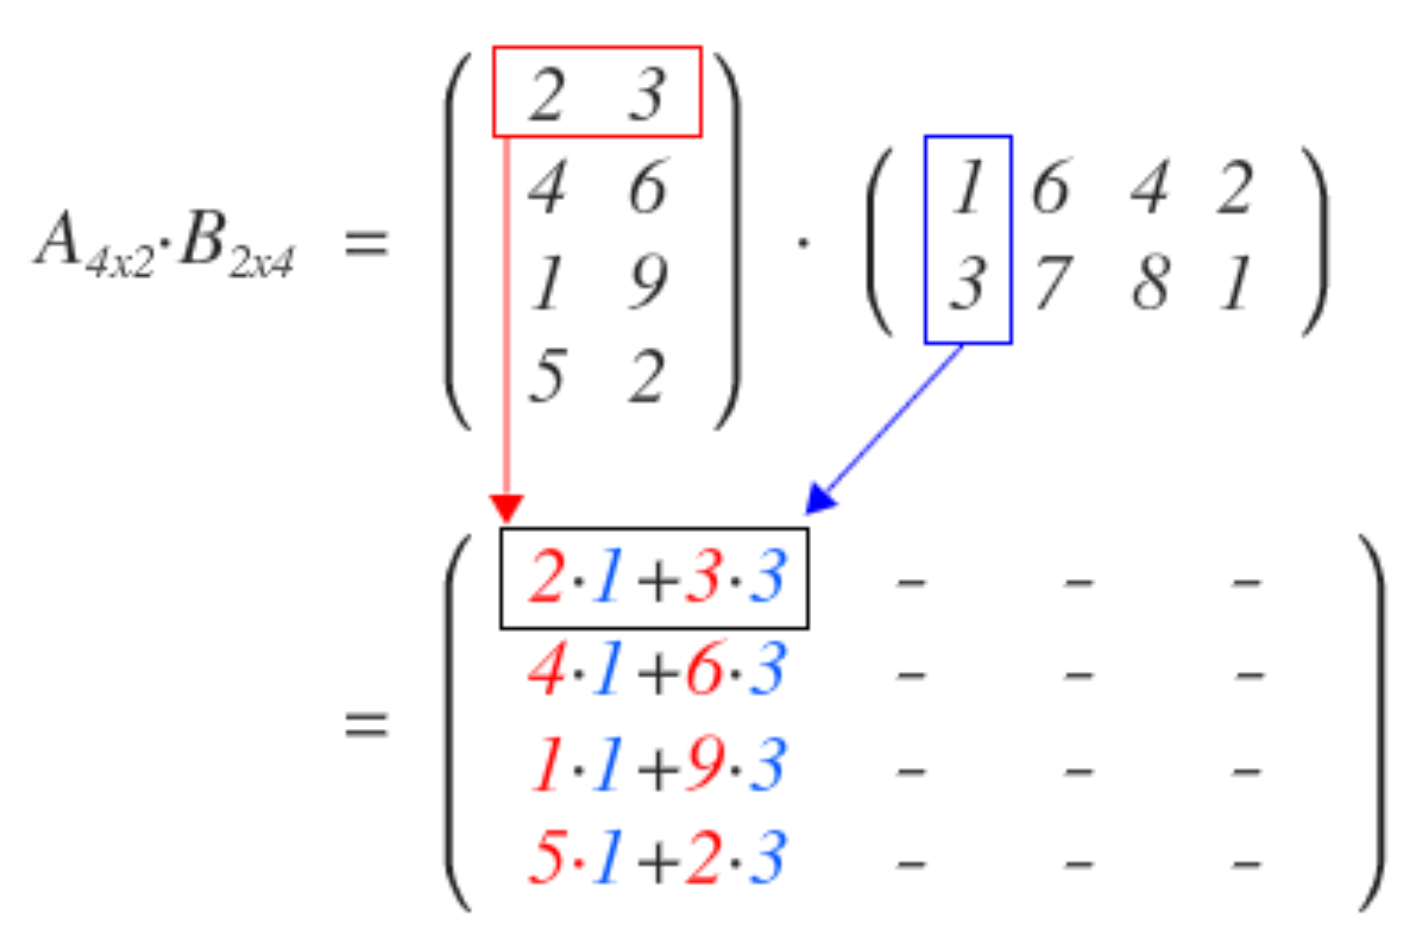
\includegraphics[width=\textwidth]{prodotto-di-matrici}
		
		\subsection{Osservazione}
			Dato un sistema composto da 3 equazioni con tre incognite, come il seguente:
			$$
			\begin{cases}
				x_1 + x_2 + x_3 = 4 \\
				2x_1 + 2x_2 + 5x_3 = 11 \\
				4x_1 + 6x_2 + 8x_3 = 24 
			\end{cases}
			$$
			
			è possibile descriverlo con due matrici: una matrice $ 3 \times 3 $, detta \textbf{matrice dei coefficienti} del sistema, descrive le incognite; mediante un vettore riga è possibile descrivere i termini noti del sistema: il sistema diviene dunque il seguente:
			$$
			A = 
			\begin{bmatrix}
				1 & 1 & 1 \\
				2 & 2 & 5 \\
				4 & 6 & 8
			\end{bmatrix}, \qquad
			b = 
			\begin{bmatrix}
				4 \\
				11 \\
				24
			\end{bmatrix}
			$$
			
			Per riottenere il sistema originale è necessario moltiplicare il sistema A con un sistema di incognite x:
			$$
			x =
			\begin{bmatrix}
				x_1 \\
				x_2 \\
				x_3
			\end{bmatrix}, \qquad
			A \cdot x =
			\begin{bmatrix}
				x_1 + x_2 + x_3 \\
				2x_1 + 2x_2 + 5x_3 \\
				4x_1 + 6x_2 + 8x_3
			\end{bmatrix}
			= b
			$$
		
		\subsection{Proprietà}
			Le proprietà del prodotto fra matrici sono le seguenti:
			\begin{enumerate}
				\item $ (AB) \cdot C = A \cdot (BC) $  associativa;
				\item $ (A + B) \cdot C = AC + BC $ distributiva;
				\item $ k \cdot (AB) = (kA) \cdot B = A \cdot (kB) \qquad \forall k \in \mathbb{R}, \forall A, B $.
			\end{enumerate}
			Com'è possibile denotare, il prodotto \textbf{non} è commutativo e dunque l'ordine delle operazioni conta (ciò non vale per tutte le coppie di matrici).
			
			\paragraph{Esempio}
			$$
			\begin{bmatrix}
				1 & 0 \\ 
				1 & 0
			\end{bmatrix}
			\begin{bmatrix}
				0 & 1 \\ 
				0& 1
			\end{bmatrix}
			=
			\begin{bmatrix}
				0 & 1 \\
				0 & 1
			\end{bmatrix}
			$$ $$ \neq $$ $$
			\begin{bmatrix}
				0 & 1 \\
				0 & 1
			\end{bmatrix}
			\begin{bmatrix}
				1 & 0 \\ 
				1 & 0
			\end{bmatrix}
			=
			\begin{bmatrix}
				1 & 0 \\ 
				1 & 0
			\end{bmatrix}
			$$
			
			\paragraph{Osservazione} Sia \textit{A} una matrice quadrata $ n \times n $ e $ k \in \mathbb{N} $ uno scalare,
			$$ A^k = \underbrace{A \cdot A \cdot ... \cdot A}_{k-volte} \text{  potenza \textit{k}-esima di \textit{A}}$$
			
			$$ A^k A^h = A^{k+h} $$
	
	\section{Tipi di matrice}
	
		\subsection{Matrice identica}
			La \textbf{matrice identica} (o \textit{matrice identità}) di ordine \textit{n} è
			$$ 
			\underbrace{I_n}_{n \times n} =
			\begin{bmatrix}
				1 & 0 & 0 & 0 \\
				0 & 1 & 0 & 0 \\
				0 & 0 & 1 & 0 \\
				0 & 0 & 0 & 1
			\end{bmatrix}_{n \times n}
			$$
			Tale matrice è simmetrica ed il suo prodotto con una matrice \textit{A} avente una dimensione uguale al lato della matrice è uguale alla matrice \textit{A}. Ciò avviene perché il prodotto fra gli elementi $ a_{ij} $ ed il corrispettivo nella matrice identità è pari ad $ a_{ij} $ stesso, gli altri prodotti sono pari all'elemento nullo.  
			$$ \implies \quad \underbrace{A}_{m \times n} \cdot I_n = A \quad \wedge \quad A \cdot I_m = A $$
		
		\subsection{Matrice invertibile}
			Sia $ A \quad n \times n $. \textit{A} è detta \textit{invertibile} se $ \exists B (n \times n) : AB = BA = I_n $.
			Se tale B esiste, si denota come $ A^{-1} $ e si chiama \textbf{matrice inversa} di \textit{A}.
		
			\paragraph{Osservazione} può valere $ AB = 0 $ con $ A \neq 0 , B \neq 0 $:
			$$
			\begin{bmatrix}
				1 & 1 \\ 
				1 & 1
			\end{bmatrix}
			\begin{bmatrix}
				1 & 1 \\ 
				-1 & -1
			\end{bmatrix}
			=
			\begin{bmatrix}
				0 & 0 \\
				0 & 0
			\end{bmatrix}
			$$
			Se \textit{A} e \textit{B} sono invertibili e sono quadrati $ n \times n \implies AB $ è invertibile:
			$$ (AB)(B^{-1}A^{-1}) = I_n $$ 
			\begin{GrayBox}
				\paragraph{Dimostrazione}
				$A (\underbrace{BB^{-1}}_{I_n}) A^{-1} = AA^{-1} = I_n $
			\end{GrayBox}
			
			$$ \implies (AB)^{-1} = B^{-1} A^{-1} $$
			$$ \implies (A_1 \cdot ... \cdot A_k)^{-1} = A_{k}^{-1} \cdot ... \cdot A_{1}^{-1} $$
			Quindi l'insieme delle \textbf{matrici $n \times n$ non invertibili} è un gruppo rispetto al prodotto matriciale (non commutativo) e viene denotato con $ GL = (n, \mathbb{R}) $ (gruppo generale lineare).
		
		\subsection{Matrice trasposta}
			Viene detta \textbf{matrice trasposta} di \textit{A} la matrice $ A^T = [a_{ji}] $ le cui righe sono le colonne di \textit{A}.
			\paragraph{Osservazione}
			\begin{itemize}
				\item $ (A + B)^T = A^T + B^T $
				\item $ (AB)^T = B^T \cdot A^T $
			\end{itemize}
		
		\subsection{Matrice simmetrica}
			Una matrice $A (n \times n) $ viene detta \textbf{simmetrica} se essa è simmetrica rispetto alla sua diagonale, ovvero se essa è uguale alla sua matrice trasposta ($ A = A^T $):
			$$
			\begin{bmatrix}
				a_{11} &
				\begin{tikzpicture}[baseline=(char.base)]
					\node(char)[draw,fill=yellow,
					shape=rounded rectangle,
					drop shadow={opacity=.5,shadow xshift=0pt},
					minimum width=1.8cm]
					{$a_{12}$};
				\end{tikzpicture} & ... & \begin{tikzpicture}[baseline=(char.base)]
					\node(char)[draw,fill=cyan,
					shape=rounded rectangle,
					drop shadow={opacity=.5,shadow xshift=0pt},
					minimum width=1.8cm]
					{$a_{1n}$};
				\end{tikzpicture}\\
				\begin{tikzpicture}[baseline=(char.base)]
					\node(char)[draw,fill=yellow,
					shape=rounded rectangle,
					drop shadow={opacity=.5,shadow xshift=0pt},
					minimum width=1.8cm]
					{$a_{21}$};
				\end{tikzpicture} & a_{12} & ... & a_{2n} \\
				... & ... & ... & a_{3n} \\
				\begin{tikzpicture}[baseline=(char.base)]
					\node(char)[draw,fill=cyan,
					shape=rounded rectangle,
					drop shadow={opacity=.5,shadow xshift=0pt},
					minimum width=1.8cm]
					{$a_{n1}$};
				\end{tikzpicture} & a_{n2} & ... & a_{nn} \\
			\end{bmatrix}
			$$
		
		\subsection{Combinazione lineare}
			Siano $ A_1, ..., A_k $ delle matrici $ m \times n $ e $ c_1, ..., c_k $ $ \in \mathbb{R} $ dei coefficienti.
			Viene detta \textbf{combinazione lineare} di $ A_1, ..., A_k $ la matrice $ m \times n $ risultante dalla somma dei prodotti delle \textit{k}-esime matrici con i \textit{k}-esimi coefficienti:
			
			$$ c_k \cdot A_k, c_k \cdot A_k, ..., c_k \cdot A_k \qquad , k \in \mathbb{N} $$
			
			\paragraph{Esempio}
			$$
			\begin{cases}
				x_1 + x_2 + x_3 = 4 \\
				2x_1 + 2x_2 + 5x_3 = 11 \\
				4x_1 + 6x_2 + 8x_3 = 24 
			\end{cases}
			\implies x_1 \begin{bmatrix}
				1 \\
				2 \\
				4
			\end{bmatrix} +  x_2 \begin{bmatrix}
				1 \\
				2 \\
				6
			\end{bmatrix} +  x_3 \begin{bmatrix}
				1 \\
				5 \\
				8
			\end{bmatrix} =  \begin{bmatrix}
				4 \\
				11 \\
				14
			\end{bmatrix} = b
			$$
		
	
	
	\section{I grafi}
	
		\begin{wrapfigure}{l}{2cm}
			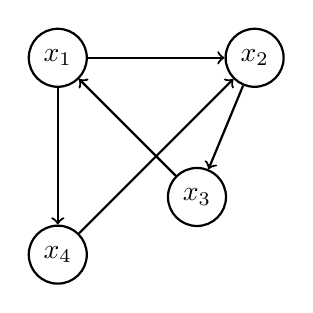
\begin{tikzpicture}[node distance={25mm}, thick, main/.style = {draw, circle}] 
				\node[main] (1) {$x_1$}; 
				\node[main] (2) [right of=1] {$x_2$}; 
				\node[main] (3) [below right of=1] {$x_3$}; 
				\node[main] (4) [below of=1] {$x_4$};  
				\draw[->] (1) -- (2);
				\draw[->] (1) -- (4);
				\draw[->] (2) -- (3);
				\draw[->] (3) -- (1);
				\draw[->] (4) -- (2);
			\end{tikzpicture}
		\end{wrapfigure}
	
		$$ V = {v_1, v_2, v_3, v_4 } \text{(insieme di vertici)} $$
		$$ E = {(1,2), (2,3), (3,1), (1,4), (4,2)} \text{(insieme dei cammini)} $$
		
		La matrice che rappresenta un grafo è denominata \textbf{matrice delle adiacenze}, tale matrice è quadrata, nelle sue righe viene indicato il peso del cammino che parte dal nodo della \textit{i}-esima riga e arriva al nodo della \textit{j}-esima colonna.
		
		$$
		A =
		\begin{bmatrix}
			0 & 1 & 0 & 1 \\
			0 & 0 & 1 & 0 \\
			1 & 0 & 0 & 0 \\
			0 & 1 & 0 & 0
		\end{bmatrix}
		$$
		
		La matrice delle adiacenze è \textit{simmetrica} se il grafo \textbf{non} è orientato.
		
		\subsection{Teorema}
			L'elemento \textit{(i, j)} della potenza $ A^{s} $ è uguale al numero di cammini di lunghezza \textit{s} dal vertice $V_i$ al vertice $V_j$.
			
			\begin{GrayBox}
				\paragraph{Dimostrazione}
				Dato $ s = 2 $ ed un nodo $V_k$, il numero di cammini di lunghezza 2 e passanti per $V_k$ è $a_{ik} \cdot a_{kj}$.
				Dato che il nodo $V_k$ può essere qualsiasi nodo ed i due nodi \textit{i} e \textit{j} sono costanti, esplicitiamo la precedente equazione rispetto ad essi:
				$$ \sum_{k=1}^n a_{ik} \cdot a_{kj} = (A^2)_{ij} $$
			\end{GrayBox}
	
	\section{Prodotto scalare in $\mathbb{R}^n$}
		Dati $x,y \in \mathbb{R}^n $, il \textbf{prodotto scalare} fra di essi è
		$$ 
		x \cdot y = \sum_{i=1}^n x_iy_i =
		\underbrace{
			\begin{bmatrix}
				x_1 & ... & x_n
			\end{bmatrix}
			\begin{bmatrix}
				y_1 \\
				... \\
				y_n
			\end{bmatrix}
		}_{\text{matrice } 1 \times 1 \implies \text{scalare}}
		=
		\begin{bmatrix}
			x_1 & ... & x_n
		\end{bmatrix}
		\begin{bmatrix}
			y_1 & ... & y_n
		\end{bmatrix}^T
		$$
		
		\subsection{Proprietà}
			\begin{enumerate}
				\item \underline{bilineare}: $ (\alpha x + \beta y) \cdot z = \alpha (x \cdot z) + \beta (y \cdot z)  $ con $ \alpha, \beta \in \mathbb{R} $ e $ x, y, z \in \mathbb{R}^n $
				\item $ x \cdot y = y \cdot x $
				\item \underline{definito positivo}: $ x \cdot x = \sum_{i=1}^n x^2_i \geq 0 $ e $ x \cdot x = 0 \iff x = 0 $
			\end{enumerate}
		
		\subsection{Norma (o lunghezza)}
			Date le precedenti proprietà è possibile definire la \textit{lunghezza} (o \textit{norma}) di $ x \in \mathbb{R}^n $ come
			$$ \Vert x \Vert = \sqrt{x \cdot x} \geq 0 $$
			Mediante la norma è dunque possibile definire pure la \textit{distanza} fra due \textit{n}-uple $x, y \in \mathbb{R}^n$ nella seguente maniera
			$$ d(x, y) = \Vert x - y \Vert \geq 0 $$
			\begin{GrayBox}
				Ciò funziona perché, facendo uso della definizione della norma e del prodotto scalare in $\mathbb{R}^2$, possiamo rappresentare tale formula come
				$$ \Vert x - y \Vert = \sqrt{(x - y)\cdot(x - y)} = \sqrt{\sum_{i=1}^{n}(x_i - y_i)^2} $$
				che è uguale alla formula che viene utilizzata per calcolare la distanza tra due punti nel piano mediante il teorema di Pitagora.
			\end{GrayBox}
		
			\paragraph{Proprietà}
			\begin{enumerate}
				\item La norma del prodotto fra una \textit{n}-upla ed uno scalare è pari al prodotto fra il modulo dello scalare e la norma della \textit{n}-upla, ovvero \newline
				$\Vert \alpha x \Vert = \vert \alpha \vert \, \Vert x \Vert $ \newline
				$\Vert \alpha x \Vert^2 = (\alpha x) \cdot (\alpha x) = \underbrace{\alpha^2}_{\sqrt{\alpha^2} = \vert \alpha \vert} \cdot \underbrace{(x \cdot x)}_{\sqrt{x \cdot x} = \Vert x \Vert} $ \newline
				Detto ciò possiamo normalizzare un vettore $v \neq 0, v \in \mathbb{R}^n$, ovvero possiamo modificarlo per far sì che la sua lunghezza sia pari ad uno:
				$$v' = \frac{1}{\Vert v \Vert} \cdot v$$
				$$\Vert v' \Vert = \frac{1}{\Vert v \Vert} \cdot \Vert v \Vert = 1$$
				$v'$ prende il nome di \textbf{versore} di \textit{v} ed è pari al rapporto fra il vettore originale e la sua lunghezza.
				\item il quadrato della lunghezza della somma di due vettori è pari alla somma fra il quadrato dei due vettori ed il doppio prodotto scalare.
				\begin{GrayBox}
					$$ \Vert x + y \Vert^2 = (x + y) \cdot (x + y) = x \cdot (x + y) + y \cdot (x + y) = x \cdot x + \underbrace{x \cdot y + y \cdot x}_{\text{doppio prodotto scalare}} + y \cdot y $$
					$$ \implies \Vert x \Vert^2 + 2 \; x \cdot y + \Vert y \Vert^2 $$
				\end{GrayBox}
				
				Lo stesso vale per il quadrato della norma della differenza fra due vettori, l'unica differenza sta nel fatto che il doppio prodotto è opposto rispetto a quello della somma (la norma di $-y$ è uguale alla norma di $y$ per la prima proprietà).
				$$ \Vert x - y \Vert^2 = \Vert x \Vert^2 - 2 \; x \cdot y + \Vert y \Vert^2 $$
				
				Dati i precedenti valori è possibile ricavare la differenza fra di essi, pari al quadruplo prodotto fra i vettori:
				$$ \Vert x + y \Vert^2 - \Vert x - y \Vert^2 = 4 \; x \cdot y $$
				
				Inoltre è possibile dire che, se \textit{x} e \textit{y} sono ortogonali, il loro prodotto è pari a 0, e dunque il quadrato della norma della somma dei due vettori è pari alla somma dei quadrati delle norme di essi (teorema di Pitagora).
				\begin{GrayBox}
					$$x \bot y \implies x \cdot y = 0 \implies \Vert x + y \Vert^2 = \Vert x \Vert^2 + \Vert y \Vert^2 $$
				\end{GrayBox}
			\end{enumerate}
			
			
			\subsection{Proiezione di un vettore su un altro vettore}
				Dati i vettori $ x, y \in \mathbb{R}^n, \quad y \neq 0 $ ed uno scalare $ c \in \mathbb{R} \ $
				$$ x - cy \, \bot \, y \implies (x - cy) \cdot y = 0 $$
				Sviluppando l'equazione risulta che lo scalare c è pari al rapporto fra il prodotto scalare fra i due vettori ed il prodotto fra il vettore nel quale si deve effettuare la proiezione per sè stesso (sappiamo, data la definizione della norma, che il prodotto di un vettore con sè stesso è pari al quadrato della sua lunghezza).
				$$ \implies x \cdot y - c \, ( y \cdot y)  = 0 $$
				$$ \implies c = \frac{x \cdot y}{y \cdot y}$$
				
				\begin{center}
					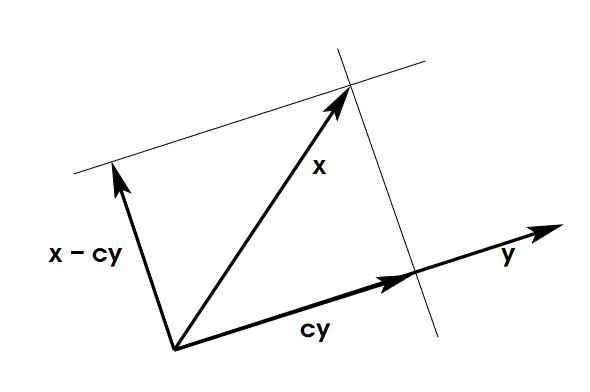
\includegraphics[width=\textwidth/2]{proiezione-vett-x-y}
				\end{center}
				
				Moltiplicando lo scalare precedentemente trovato con il vettore nel quale deve essere effettuata la proiezione, è possibile ottenere la \textbf{proiezione ortogonale} su x su y, chiamato anche \textit{vettore proiezione}.
				$$ pr_y(x) = c \cdot y = \frac{x \cdot y}{\Vert y \Vert^2} \cdot y \in \mathbb{R}^n $$
			
			\subsection{Disuguaglianza di Cauchy-Schwanz}
				Tale disuguaglianza afferma che il modulo del prodotto fra due vettore è minore (o uguale) al prodotto fra le norme dei vettori.
				$$ \vert x \cdot y \vert \leq \Vert x \Vert \cdot \Vert y \Vert \qquad \forall x, y \in \mathbb{R}^n $$
				I termini risultano uguale se e solo \textit{x} e \textit{y} sono proporzionali, ovvero 
				$$ x = \lambda \cdot y \, , \; \forall \lambda \in \mathbb{R} $$
				
				\begin{GrayBox}
					\paragraph{Dimostrazione} se $ y = 0 \implies \text{i due termini sono uguali} $ \newline
					se $ y \neq 0 \implies x = pr_y(x) + x' \, , \; \text{con } x' \bot y $ \newline
					detto ciò sappiamo che la norma di \textit{x} sarà sicuramente maggiore della norma della sua proiezione su \textit{y}, dato che essa è una degli addendi che generano x; Definito ciò possiamo dunque dire che il quadrato della norma di \textit{x} è maggiore del quadrato della norma di tale proiezione.
					$$ \Vert x \Vert^2 = \Vert pr_y(x) \Vert^2 + \Vert x' \Vert^2 \geq \Vert pr_y(x) \Vert^2 = \Vert \frac{x \cdot y}{\Vert y \Vert^2} \cdot y \Vert^2$$
					Semplificando la proiezione è possibile dire che il quadrato della norma di \textit{x} è maggiore (o uguale) al rapporto fra il quadrato del modulo del prodotto fra \textit{x} e \textit{y} e il quadrato della norma di \textit{y}.
					$$ \Vert x \Vert^2 \geq \frac{\vert x \cdot y \vert^2}{\Vert y \Vert^4} \cdot \Vert y \Vert^2 = \frac{\vert x \cdot y \vert^2}{\Vert y \Vert^2} $$
					
					Portando a sinistra il denominatore del secondo termine e mettendo tutto sotto radice, è possibile sostenere l'assunto iniziale, ovvero
					$$ \vert x \cdot y \vert \leq \Vert x \Vert \cdot \Vert y \Vert \qquad \forall x, y \in \mathbb{R}^n $$
				\end{GrayBox}
			
			\subsection{Disuguaglianza triangolare}
				Viene affermato che la lunghezza della somma di due vettori è minore (o uguale) alla somma delle loro lunghezze.
				$$ \Vert x + y \Vert = \Vert x \Vert + \Vert y \Vert \quad x, y \in \mathbb{R}^n $$
				\begin{GrayBox}
					\paragraph{Dimostrazione} La dimostrazione di questo assunto è abbastanza semplice perché sappiamo che il quadrato della lunghezza di due vettori è pari alla somma dei quadrati delle loro lunghezze ed il loro doppio prodotto, i due termini saranno uguali nei casi nei quali il doppio prodotto è nullo, ovvero quando i due vettori sono perpendicolari.
				\end{GrayBox}
				
				\subsection{Disuguaglianza triangolare per la distanza}
				La distanza fra due vettori \textit{x} e \textit{y} è sempre minore (o uguale) alla distanza fra di essi passando per un vettore \textit{z}:
				$$ d(x, y) \leq d(x, y) + d(z, y) \qquad \forall x, y, z \in \mathbb{R}^n $$
			
				\begin{GrayBox}
					La distanza fra \textit{x} e \textit{y} può essere vista come la somma della differenza fra \textit{x} e \textit{z} e la differenza fra \textit{z} e \textit{y}:
					$$ d(x, y) = \Vert x - y \Vert = \Vert (x - z) + (z - y) \Vert $$
					Invece, la distanza fra \textit{x} e \textit{y} calcolata passando per un vettore \textit{z} è pari alla somma fra la lunghezza del segmento \textit{xz} ed il segmento \textit{zy}:
					$$ d(x, z) + d(z, y) = \Vert x - z \Vert + \Vert z - y \Vert $$
					Facendo uso della disuguaglianza triangolare precedentemente dimostrata, è possibile affermare la seguente:
					$$ \Vert (x - z) + (z - y) \Vert \leq \Vert x - z \Vert + \Vert z - y \Vert $$
					E da ciò ne conviene l'assunto iniziale.
				\end{GrayBox}
			
			\subsection{Angolo compreso tra due vettori}
				Date le \textit{n}-uple \textit{x} e \textit{y} \underline{non nulle}, e sapendo che il rapporto fra il prodotto vettoriale $ x \cdot y $ ed il prodotto $ \Vert x \Vert \cdot \Vert y \Vert $ è compreso fra -1 e 1 \footnote{la disuguaglianza di Cauchy-Schwanz afferma che il modulo del primo è minore del secondo, dunque senza modulo il risultato di tale prodotto è compreso fra -1 e 1}, è possibile affermare che il risultato di tale prodotto è pari al coseno dell'angolo (convesso) compreso fra i due vettori.
				\begin{GrayBox}
					$$ -1 \leq \frac{x \cdot y}{\Vert x \Vert \cdot \Vert y \Vert} \leq 1 $$
					$$ \implies \cos \theta = \frac{x \cdot y}{\Vert x \Vert \cdot \Vert y \Vert} \: , \quad \theta \in [0, \pi] $$
				\end{GrayBox}
\chapter{Distanze}
	\section{Distanza punto - piano}
		Dati un piano ed un punto nello spazio definiti come i seguenti:
		$$ \pi = ax + by + cz = d \: , \qquad P_0=(x_0, y_0, z_0) $$
		La distanza fra di essi è pari a
		$$ d(P_0, \pi) = \frac{\vert a x_0 + by_0 + cz_0 - d \vert}{\sqrt{a^2 + b^2 + c^2}} $$
		\begin{GrayBox}
			\paragraph{Dimostrazione}
			\begin{center}
				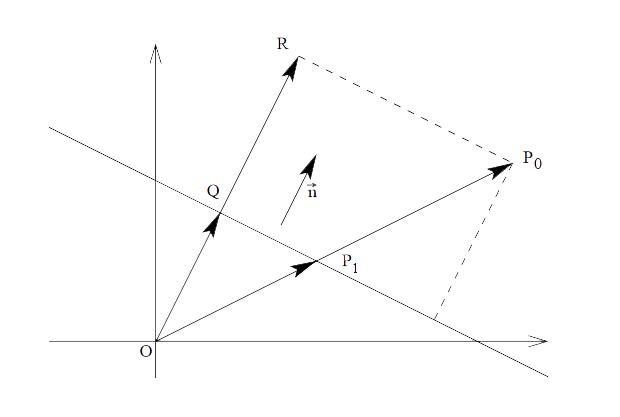
\includegraphics[width=\textwidth]{distanza-punto-piano}
			\end{center}
			La distanza fra il punto ed il piano è pari alla lunghezza del segmento $ \overrightarrow{QR} $: tale segmento non è altro che la proiezione di $ \overrightarrow{P_1P_0} $ nel versore normale \textit{n} del piano \footnote{$ \vec{n} = \frac{(a, b, c)}{\sqrt{a^2 + b^2 + c^2}} = (\frac{a}{\sqrt{a^2 + b^2 + c^2}}, \frac{b}{\sqrt{a^2 + b^2 + c^2}}, \frac{c}{\sqrt{a^2 + b^2 + c^2}})$  è il versore normale del piano (la sua lunghezza, per definizione, è pari ad uno}.
			$$ d (P_0, \pi) = \Vert \overrightarrow{QR} \Vert = \Vert pr_{\vec{n}}(\overrightarrow{P_1P_0}) \Vert $$
			Ricordando che la formula per trovare la proiezione di un vettore su un altro è $ pr_y(x) = \frac{x \cdot y}{\Vert y \Vert^2} \cdot y $, la lunghezza della proiezione di $ \overrightarrow{P_1P_0} $ è
			$$ pr_{\vec{n}}(\overrightarrow{P_1P_0}) = \frac{\overrightarrow{P_1P_0} \cdot \vec{n}}{\Vert \vec{n} \Vert^2} \cdot \vec{n} $$
			Dato che, per definizione, la lunghezza del versore $\vec{n}$ è 1, il denominatore di tale equazione viene sottinteso essere uguale ad 1.
			$$ d(P_0, \pi) = \vert \overrightarrow{P_1P_0} \cdot \vec{n} \vert $$
			Il risultato di tale prodotto vettoriale è il seguente:
			$$ \vert \overrightarrow{P_1P_0} \cdot \vec{n} \vert = \Big\vert \frac{a \cdot (x_0 - x_1) + b \cdot (y_0 - y_1) + c \cdot ( z_0 - z_1 )}{\sqrt{a^2 + b^2 + c^2}} \Big\vert $$
			Dato che $P_1$ può essere un punto qualsiasi nel piano, il prodotto fra le coordinate del piano e quelle di tale punto possono essere raggruppate nell'intercetta $d$:
			$$ d (P_0, \pi) = \frac{\vert a x_0 + b y_0 + c z_0 - d \vert}{\sqrt{a^2 + b^2 + c^2}} $$
			Nel piano la distanza fra un punto ed una retta è analoga alla precedente, viene esclusa la terza dimensione
			$$ d (P_0, r) = \frac{\vert a x_0 + b y_0 - c \vert}{\sqrt{a^2 + b^2}} \quad , \text{ con } r = ax + by = c $$
		\end{GrayBox}

	\section{Distanza punto - retta}
		Dati una retta ed un punto nello spazio, per poter trovare la distanza fra di essi è necessario ottenere il piano ortogonale alla retta e passante per il punto; la distanza fra il punto di intersezione tra il piano e la retta ed il punto iniziale sarà pari alla distanza fra quest'ultimo e la retta.
		
		\begin{GrayBox}
			\paragraph{esempio}
			Dati
			$$ P_0 = (1, 2, 1) \qquad \qquad r = \begin{cases}
				x = 2t \\
				y = t \quad , \: t \in \mathbb{R} \\
				z = t
			\end{cases} $$
		trovare la distanza fra di essi.
		
		\begin{enumerate}
			\item ricavo la normale al piano $ \pi \bot r \, : \, P_0 \in \pi $:  $ \vec{v} = (2, 1, 1) $
			\item scrivo l'equazione del piano facendo uso della normale e delle coordinate del punto P: $ \pi = 2 \cdot (x - 1) + (y - 2) + (z - 1) = 0 $
			\item sostituisco le coordinate di \textit{r} all'interno dell'equazione del piano per trovare la loro intersezione \textit{Q}:
			$$ Q : \, 2 (2t - 1) + (t - 2) + (t - 1) = 0 \implies t = 5/6 $$
			$$ \text{sostituisco... } Q = (\frac{5}{3}, \frac{5}{6}, \frac{5}{6}) $$
			\item la distanza fra $P_0$ e \textit{Q} è pari a quella fra $P_0$ ed r:
			$$ d (P_0, r) = d (P_0, Q) = \Vert \overrightarrow{P_0Q} \Vert = ... $$
		\end{enumerate}
		\end{GrayBox}
	\section{Distanza fra rette parallele nello spazio}
		\subsection{nello spazio}
			la distanza fra di esse è pari alla distanza fra i loro punti di intersezione con il piano $\pi$ a loro ortogonale.
			
		\subsection{nel piano}
			la distanza fra di esse è pari a quelli che vi è fra i loro punti di intersezione con una retta a loro parallela ($ m_s = - \frac{1}{m_r} $).
	
	\section{Distanza fra rette sghembe}
		Date le rette $r$ e $r'$, vi sono due metodi per trovare la distanza fra di esse.
		
		\subsection{I metodo}
			Definiamo i punti $P \in r$ e $Q \in r'$ le cui coordinate sono pari alle coordinate parametriche delle due rette.
			
			Troviamo il vettore $\overrightarrow{PQ}$ e, dato che quest'ultimo deve essere perpendicolare alle due rette, il suo prodotto vettoriale con i vettori direttori delle rette deve essere pari a 0.
			$$ \begin{cases}
				\overrightarrow{PQ} \cdot \vec{v} = 0 \\
				\overrightarrow{PQ} \cdot \vec{v'} = 0
			\end{cases}$$
		
			Risolvendo tale sistema è possibile trovare i due parametri \textit{t} ed \textit{s}, relativi rispettivamente alle rette \textit{r} e \textit{r'}; sostituendo tali parametri nei punti \textit{P} e \textit{Q}, è possibile trovare le coordinate dei due punti la cui distanza è pari a quella fra le due rette sghembe.
		
		\subsection{II metodo}
			Definisco il fascio dei piani contenenti \textit{r'}:
			$$ \lambda \cdot (\text{eq. cartesiana 1}) + \mu \cdot (\text{eq. cartesiana 2}) = 0 $$
			Il piano che dobbiamo identificare deve essere parallelo a \textit{r}, dunque la sua normale (le cui coordinate sono pari ai coefficienti nell'equazione del fascio) deve essere perpendicolare alla direttrice di \textit{r}
			$$ \pi \parallel r \iff \vec{n} \bot \vec{v} \iff \vec{n} \cdot \vec{v} = 0 $$
			Facendo ciò è possibile trovare la relazione che lega i due parametri $\lambda$ e $\mu$, fissandone uno sarà possibile trovare anche l'altro.
			
			Una volta sostituiti i due parametri nell'equazione del fascio di piani sarà possibile ottenere il piano che cercavamo, la sua distanza da un punto $P_0 \in r$ è pari a quella fra le due rette sghembe.
\chapter{Sistemi lineari}
	Data una matrice composta da \textit{m} equazioni lineari in $ x1 ... x_n $
	$$ \begin{cases}
		a_{11} x_1 + a_{12} x_2 + ... + a_{1}n x_n = b_1 \\
		a_{21} x_1 + a_{22} x_2 + ... + a_{2n} x_n = b_2 \\
		... \\
		a_{m1} x_1 + a_{m2} x_2 + ... + a_{mn} x_n = b_m
		\end{cases} = 
		\underbrace{A}_{m \times n}\underbrace{x}_{n \times 1} = \underbrace{b}_{m \times 1} $$
		
		Dove
		
		$$ A = [a_{ij} ] \text{ è la matrice dei coefficienti} $$
		$$ b = \begin{bmatrix}
			b1 \\
			... \\
			b_m
		\end{bmatrix} \text{ è il vettore dei termini noti} $$
	 $$ x = \begin{bmatrix}
	 	x_1 \\
	 	... \\
	 	x_m
	 \end{bmatrix}$$
	
	$ \underbrace{(Ab)}_{m \times (n + 1)} $ viene detta \emph{matrice completa} del sistema ed è risultante dalla concatenazione di \textit{A} con \textit{b}.
	
	\paragraph{Esempio}
	\lipsum[2-4]
	
	\section{Operazioni elementari sulle righe di (Ab)}
		\begin{enumerate}[(I)]
			\item Scambio delle righe \textit{i} e \textit{j}
			$$ S_{ij}$$
			\item Moltiplicazione di una riga, la \textit{i}-esima, per uno scalare $ c \neq 0 $
			$$ D_i(c) $$
			\item Somma della \textit{i}-esima riga con la \textit{j}-esima riga moltiplicata per \textit{c}
			$$ E_{ij}(c) $$
		\end{enumerate}
		
		\paragraph{Osservazione}
		Ognuna delle operazioni è reversibile:  \newline
		\begin{enumerate}[(I)]
			\item $ S_{ij}^{-1} = S_{ij} $
			\item $ D_{i}^{-1}(c) = D_{i}(\nicefrac{1}{c}) $
			\item $ E_{ij}^{-1}(c) = E_{ij}(-c) $
		\end{enumerate}
		
		\subsection{Matrice equivalente per righe} 
			Prende il nome di \textbf{matrice equivalente per righe}, rispetto ad una matrice \textit{A}, se è risultante da essa mediante una \emph{successione} di operazioni elementari.
			
			Data una matrice $ (Ab) $, le soluzioni di $ Ax = b $ lo sono anche per le sue equivalenti per righe $ A'x = b' $.
			
		\subsection{Matrice a scalini}
			Una matrice \textit{A} viene detta \underline{a scalini} se il numero di zeri che precede il 1° elemento non nullo, detto \textbf{pivot}, aumenta dalla prima all'ultima riga. Questo tipo di matrice è risolubile quando l'ultima colonna (\textit{b} di $(Ab) $ ) non contiene pivot (nel caso contrario avremmo l'uguaglianza falsa $ 0 = b_m $ ).
		
		\subsection{Matrice ridotta}
			Una matrice scalini viene detta \underline{ridotta} quando i suoi pivot sono tutti pari ad 1 e sono gli unici elementi non nulli all'interno della propria colonna.
			\paragraph{Esempio} 
			$$
			\begin{bmatrix}
			1 & 0 & 0 & 3 \\
			0 & 1 & 0 & 9 \\
			0 & 0 & 1 & -2 
			\end{bmatrix} \implies
			\begin{cases}
				x = 3 \\
				y = 9 \\
				x = -1
			\end{cases} \implies \text{Sol}(Ax=b) = {(3, 9. -2)}
			$$
	
	\section{Riduzioni a scala}
		\paragraph{Teorema} Ogni matrice $ A (m \times n) $ è equivalente per righe ad una matrice a scalini \textit{S}, ridotta.
		
		\begin{GrayBox}
			\subsection{Dimostrazione}
			\paragraph{I caso}: la $1^a$ colonna \textbf{non} è nulla.
			Sia $ a_{i1} \neq 0 $, è possibile, non facendo alcuno scambio, supporre che $ a_{11} \neq 0 $ (pivot).
			Con l'operazione $ E_{i1}(\nicefrac{-a_{i1}}{a_{11}}) \: , \: i \geq 2 $ è possibile annullare tutti gli elementi della $1^a$ colonna al di sotto di $a_{11}$.
			Si ripete tale procedimento sulla matrice ottenuta togliendo la $1^a$ riga e $1^a$ colonna.
			
			\paragraph{II caso}: la prima colonna è nulla, si ripete il precedente procedimento togliendo la prima colonna.
			
			La matrice ottenuta è a scalini; è possibile svolgere delle operazioni elementari su di essa per ottenere la matrice a scalini ridotta \textit{S}, tali operazioni sono $ D_i(\nicefrac{1}{p_i}) $, con \textit{p} pivot della \textit{i}-esima riga, e $ E_{ij}(c) $.
			
		\end{GrayBox}
		
		\subsection{rango di una matrice}
			Viene detto \emph{rango} (o \emph{caratteristica} di una matrice \textit{A} il numero di pivot in una (qualsiasi) matrice equivalente ad \textit{A}.
			$$ \underbrace{0}_{ A \, = \, 0 } \leq rg(A) \leq min(m, n) $$
		
	\section{Sistema risolubile}
		un sistema $ Ax = b $ si dice \textbf{risolubile}, o \textbf{compatibile}, quando ogni matrice a scalini ottenuta da $(Ab)$ \underline{non} ha pivot nell'ultima colonna.
		
		\begin{align}
		(Ab) \rightarrow (A'b') & =
		\begin{bmatrix}
			0 & \dots & p_1 & \dots & \dots & \dots & * \\
			0 & \dots & \dots & p_2 & \dots & \dots & * \\
			0 & \dots & \dots & \dots & \dots & p_r & * \\
			0 &  &  & \dots &  &  & 0  
		\end{bmatrix} \notag \\
		\text{\textbf{oppure} } (A'b') & = 
		\begin{bmatrix}
			0 & \dots & p_1 & \dots & \dots & \dots & * \\
			0 & \dots & \dots & p_2 & \dots & \dots & * \\
			0 & \dots & \dots & \dots & \dots & \dots & \color{red} p_r \\
			0 &  &  & \dots &  &  & 0  
		\end{bmatrix} \notag
		\end{align}
		
		Se il sistema è risolubile, ci sono $n-r$ \underline{variabili libere} (corrispondenti alle colonne non contenenti alcun pivot) e \textit{r} \underline{variabili dipendenti} ($ r = rg (Ab) $).
		
		\subsection{Teorema di Ronché - Capelli}
			\begin{enumerate}[(a)]
				\item $ Ax = b $ è risolubile 
				
				$ \iff rg (Ab) = rg (A) $: nel primo caso, fra quelli precedentemente citati, è \textit{r}, nel secondo è \textit{r - 1}.
				\item sia $ Ax = b $ risolubile, la soluzione è unica se, e solo se, il suo rango è pari al rango di \textit{A}.
				
				Se il rango di \textit{A} è minore (o uguale) al numero delle sue colonne, ci sono infinite soluzioni dipendenti dai $ n - rg(A) $ parametri.
			\end{enumerate}
			\paragraph{nullità di una matrice}: è il numero $ n - rg(A) = null(A) $ delle variabili libere di \textit{A}.  
			
	\section{Sistemi omogenei}
		$$ Ax = 0 $$
		
		I sistemi omogenei sono:
		\begin{enumerate}
			\item sicuramente risolubili perché $ x = 0 $ è sempre una soluzione.
			\item se $ Ax = 0 $ e $ Ay = 0 $
			$$ \implies A ( x + y ) = Ax + Ay = 0 + 0 = 0 $$
			dato lo scalare \textit{c}, $ A(cx) = c \cdot (Ax) = c \cdot 0 = 0 $.
			\begin{GrayBox}
				in un piano, la soluzione di un sistema omogeneo è una retta, mentre nello spazio tale soluzione può essere una retta o un piano. In tutti i casi la soluzione deve passare per l'origine.
			\end{GrayBox}
		\end{enumerate}
		
		\subsection{Relazione con i sistemi non omogenei}
			Sia $ Ax = b $ risolubile, e sia \textit{y} una soluzione particolare, allora la soluzione del primo sistema può essere vista come la soluzione di un sistema omogeneo $ Ax_0 = 0 $ traslato di \textit{y}.
			$$ \text{Sol} (Ax = b) = \{ x = y + x_0 \; \vert \; Ax_0 = 0 \} $$ 
			
			\begin{GrayBox}
				\paragraph{Dimostrazione} 
				$$ Ax = 0 \implies A (y + x_0) = Ay + Ax_0 = b + 0 = b $$
				$$ Ax = b \implies A ( x - y ) = Ax - Ay = b - b = 0 $$
				$$ \implies x - y =: x_0 \in \text{Sol} ( Ax = 0 ) $$
				$$ \iff x = y + x_0 $$ 
			\end{GrayBox}
		
		\subsection{Operazioni elementari come prodotto matriciale}
			Dato una matrice $ \underset{m \times n}{A} $, l'applicazione di un'operazione elementare su di essa può essere vista come il suo prodotto con una matrice che prende il nome di \textbf{matrice elementare}, le matrici elementari sono le seguenti:
			\begin{enumerate}[(I)]
				\item $ S_{ij} \implies \underset{m \times m}{S_{ij}} \cdot \underset{m \times n}{A} $ \newline
				La matrice $S_{ij}$ è ottenuta da $I_m$ eseguendo lo scambio delle righe \textit{i} e \textit{j}.
				\begin{GrayBox}
					\paragraph{Esempio}
					$$
					\underset{S_{12}}{\begin{bmatrix}
						0 & 1 & 0 \\
						1 & 0 & 0 \\
						0 & 0 & 1
					\end{bmatrix}}
					\cdot \underset{3 \times n}{\begin{bmatrix}
						A_1 \\
						A_2 \\
						A_3
					\end{bmatrix}} = \begin{bmatrix}
						A_2 \\
						A_1 \\
						A_3
					\end{bmatrix}
					$$
				\end{GrayBox}
				\item $ D_i(c) \implies D_i(c) \cdot A $ \newline
				La matrice $D_i(c)$ è ottenuta da $I_m$ moltiplicando la riga \textit{i}-esima per \textit{c}.	
				\begin{GrayBox}
					\paragraph{Esempio}
					$$
					\underset{\text{matrice diagonale}}{\begin{bmatrix}
							1 & & \dots & & 0 \\
							  & \ddots & &  & \\
							\vdots & & c &  & \vdots  \\
							  & & &  \ddots &  \\
							0 & & \dots & & 1
					\end{bmatrix}}
					\cdot \underset{3 \times n}{\begin{bmatrix}
							A_1 \\
							\vdots \\
							A_i \\
							\vdots \\
							A_m
					\end{bmatrix}} = \begin{bmatrix}
						A_1 \\
						\vdots \\
						c \cdot A_i \\
						\vdots \\
						A_m
					\end{bmatrix}
					$$
				\end{GrayBox}
				\item $ E_ij(c) \implies E_ij(c) \cdot A $ \newline
				\begin{GrayBox}
					\paragraph{Esempio}
					$$
					\NiceMatrixOptions{code-for-last-row=\scriptstyle,code-for-last-row=\scriptstyle}
					\underset{m \times n}{E_{ij}(c)} =\begin{bNiceMatrix}[last-row,last-col=6]
						1 & & \dots & & 0 & \\
						  & \ddots & & & & \\
						0 & \dots & 1 & \dots & c & i \\
						  & & & \ddots & & \\
						  0 & & \dots & & 1 & \\
						  & & i & & j & \\
					\end{bNiceMatrix} \qquad (\text{con } i \neq j)
					$$
				\end{GrayBox}
			\end{enumerate}	
			
			le \underline{matrici elementari}, sono invertibile come le operazioni a loro corrispondenti e con le stesse matrici rappresentate dall'inversa di tali operazioni ($ S_{ij} \, , \, D_i(\nicefrac{1}{c}) \, , \, E_{ij}(-c)$).
		
		
		\subsection{Proposizione} \label{proposizone_sistemi_lineari}
			Sia \textit{A} ($m \times n$) una matrice con due dimensioni differenti, esiste una matrice quadrata invertibile \textit{P} ($m \times m$) tale che $PA = S$ a scalini.
			Se \textit{A} fosse una matrice quadrata ($m = n$) ed il suo rango fosse il massimo ($rg(A) = n$), allora la sua versione ridotta sarebbe pari alla matrice identica con la sua stessa dimensione.
			$$ m = n \wedge rg(A) = n \implies rreff(A) = I_n $$
			
			Se il prodotto fra \textit{P} ed \textit{A} fosse uguale alla matrice ridotta associata ad \textit{A}, allora \textit{A} sarebbe invertibile e la sua inversa sarebbe \textit{P}.
			$$ PA = rreff(A) \implies A^{-1} = P $$
			
			\begin{GrayBox}
				\paragraph{Dimostrazione} se $ E_k \dots E_1 A = S $ a scalini
				$$ \implies P = E_k \dots E_1 \text{ è invertibile, perché è prodotto di matrici elementari invertibili} $$
				$$ \implies P^{-1} = E_1^{-1} \dots E_k^{-1} $$
				Se $m = n$ e il rango di \textit{A} è il massimo, la matrice ridotta associata ad \textit{A} è pari alla matrice identica di dimensione \textit{n}.
				
				Dato che $ PA = rreff(A) $ e $ rreff(A) = I_n $, ci è possibile dire che $ PA = I_n $.
				
				$$ P^{-1} (PA) = P^{-1} I_n $$
				$$ A = \underbrace{I_n}_{P \cdot P^{-1}} A = P^{-1} $$
				$$ \iff AP = P^{-1} P = I_n $$ 
			\end{GrayBox}
		
		\subsection{Teorema}
			\begin{enumerate}[(a)]
				\item se $\underset{ n \times n }{A}$ è invertibile $ \implies $ ogni sistema $ Ax = b $ ha una soluzione unica (perché il rango è massimo);
				\begin{GrayBox}
					\paragraph{Dimostrazione}
					\underline{Se} x è soluzione del sistema $(Ax=b)$, possiamo moltiplicare ambo i membri del sistema con l'inversa di \textit{A}. Nel primo membro rimarrà solo il vettore delle incognite, uguale al prodotto fra il vettore dei termini noti e l'inversa di \textit{A};
					$$ A^{-1} \cdot (Ax) = A^{-1} b \implies x = A^{-1} b $$
					Sostituendo tale \textit{x} all'interno del sistema $Ax=b$ otteniamo l'identità $b=b$, ovvero una conferma dell'unicità della soluzione.
					$$ A (A^{-1}b) = b \implies b = b \implies x = A^{-1} b \text{ è l'unica soluzione}$$
				\end{GrayBox}
			
				\item $A (n \times n) $  è invertibile $\iff rg(A) = n $; 
				\begin{GrayBox}
					\paragraph{Dimostrazione}
					Facendo uso della proposizione \ref{proposizone_sistemi_lineari} è possibile dire, per ipotesi, che, quando la matrice \textit{A} è invertibile, il suo rango è massimo; da ciò possiamo aggiungere che vi è un'unica soluzione (punto a). Dato che la matrice ha un'unica soluzione, la sua nullità e nulla ed il rango è massimo: ($ null(A) = n- rg(A) = 0 $).
				\end{GrayBox}
			\end{enumerate}
		
			Se concatenassimo \textit{A} con la matrice identica avente le sue stesse dimensioni, e moltiplicassimo tale matrice completa $(n \times 2n)$ con l'inversa di \textit{A}, \textit{P}, sarebbe possibile ottenere il rango di \textit{A}.
			$$ \underset{n \times n}{P} \cdot \underset{n \times 2n}{(A \, I_n)} = rref(A \, I_n) $$
			
		\subsection{Studio del rango di una matrice}
			Data una matrice \textit{A} ($n \times n$), durante lo studio del suo rango si può incorrere in due casi differenti:
				\paragraph{I caso} ci sono meno di \textit{n} pivot nelle prime \textit{n} colonne: \newline
				In questo caso è possibile sostenere che, dato $rg(A) < n$, la matrice \textbf{non} è invertibile.
				$$ rg(A) < n \implies \nexists A^{-1} $$
				
				\paragraph{II caso} ci sono \textit{n} pivot nelle prime \textit{n} colonne: \newline
				Esiste l'inversa della matrice originale.
				$$ rg(A) = n \implies \exists A^{-1} $$

\chapter{Spazi vettoriali}

	Uno spazio vettoriale è quella figura algebrica composta da:
	\begin{enumerate}
		\item un gruppo commutativo $(V, +)$, i cui elementi sono detti \textit{vettori};
		\item un campo $\mathbb{K}$;
		\item una funzione detta \underline{prodotto esterno} (o prodotto di uno scalare per un vettore).
		$$ f \, : \mathbb{K} \times V \rightarrow V $$
		$$ 	\qquad \qquad \qquad \quad (k, v) \rightarrow f(k, v) = kv $$
	\end{enumerate}
	
	\section{Proprietà}
		Tale figura algebrica, per essere considerata uno spazio vettoriale, deve soddisfare le seguenti proprietà:
		\begin{enumerate}[(1)]
			\item Proprietà distributiva del prodotto esterno rispetto alla somma di scalari: $ (k_1 + k_2 ) v = k_1v + k_2v $
			\item Proprietà distributiva del prodotto esterno rispetto alla somma di vettori: $ k(v_1 + v_2) = kv_1 + kv_2 $
			\item Proprietà associativa del prodotto esterno: $ (k_1 k_2) v = k_1 (k_2v) $
			\item Esistenza dell'identità rispetto al prodotto esterno: $ 1v = v $
		\end{enumerate}
		$ \forall k, k_1, k_2 \in \mathbb{K}, \quad \forall v, v_1, v_2 \in V $

		\paragraph{Esempi}
		\begin{enumerate}[(1)]
			\item $ V^2, v^3 $ sono vettori geometrici $ (\mathbb{K} = \mathbb{R}) $
			\item $ \underset{\text{spazio vettoriale \textbf{reale}}}{\mathbb{R}^n} \quad (\mathbb{K} = \mathbb{R}) $
			\item $ \underset{\text{spazio vettoriale \textbf{complesso}}}{\mathbb{C}^n} \quad (\mathbb{K} = \mathbb{C}) $
		\end{enumerate}

	\section{Sottospazi vettoriali}
		Sia $\mathbb{V}$ uno spazio vettoriale su $\mathbb{K}$.
		Un sottoinsieme \emph{non vuoto} $ \mathbb{W} \subseteq \mathbb{V} $ viene detto sottospazio vettoriale di $\mathbb{V}$ se è chiuso rispetto alla somma di vettori ed al prodotto esterno, ovvero:
		\begin{enumerate}[(1)]
			\item $ w_1 + w_2 \in \mathbb{W} \, , \qquad \forall w_1, w_2 \in \mathbb{W} $
			\item $ kw \in \mathbb{W} \, , \quad \forall k \in \mathbb{K}, \forall w \in \mathbb{W} $
		\end{enumerate}
		Detto ciò è possibile dire che anche $\mathbb{W}$ contiene il vettore nullo $0v$ di $\mathbb{V}$ ed anche $\mathbb{W}$, essendo sottospazio di $\mathbb{V}$, è uno spazio vettoriale sul campo $\mathbb{K}$.

	\section{Dipendenza e indipendenza lineare}
		\subsection{Combinazione lineare di vettori}
			La combinazione lineare di \textit{k} vettori $v_1, \dots, v_k \in \mathbb{V} $ con coefficienti $ c_1, \dots, c_2 \in \mathbb{K} $ è il vettore $$ v = \sum_{i=1}^{k} c_i \cdot v_i = c_1v_1 + \dots + c_kv_k \in \mathbb{W} $$
			
			\begin{GrayBox}
				\paragraph{Esempi}
				\begin{enumerate}
					\item la terna di numeri reali $(a, b, c) \in \mathbb{R}^3 $ è combinazione lineare dei vettori $(1, 0, 0), (0, 1, 0), (0, 0, 1)$ mediante i coefficienti $a, b, c \in \mathbb{R}$.
					\item dati i seguenti elementi dello spazio $\mathbb{R}[x]$:
					$$ p_1(x) = x^2 - x + 1 $$
					$$ p_2(x) = x^3 + 2 $$
					e facendo uso dei coefficienti $c_1 = 2 \, , \, c_2 = -1 $, la combinazione lineare che risulta è la seguente:
					$$ p(x) = 2 \cdot p_1(x) - 1 \cdot p_2(x) = 2x^2 - 2x + 2 - x^3 - 2 = -x^3 + 2x^2 - 2x $$ 
				\end{enumerate}
			\end{GrayBox}
			
			\paragraph{Osservazione} dato $ \mathbb{W} \subseteq \mathbb{V} $ non vuoto, esso è un sottospazio di $\mathbb{V}$ se e solo se $\mathbb{W}$ contiene tutte le combinazioni lineari ottenute a partire da elementi di $\mathbb{W}$ (e dunque è "chiuso" anche rispetto alla combinazione lineare).
			
		\subsection{Vettori dipendenti o indipendenti}
			Un insieme di vettori $ \{ v_1, \dots, v_2 \} \in \mathbb{V} $ si dice \textbf{linearmente dipendente} se almeno uno di essi è combinazione lineare degli altri; al contrario, si dicono \textbf{linearmente indipendenti} quando il vettore nullo dello spazio può essere scritto come combinazione lineare di tali vettori \underline{solo} c on coefficienti tutti nulli.
			
			In sintesi:
			\begin{enumerate}
				\item $ c_1v_1 + \dots + c_kv_k = 0 \implies c_1 = c_{\dots} = c_k = 0 $
				\item se $ v_1, \dots, v_k $ sono linearmente dipendenti:
					\begin{enumerate}
						\item $ \implies c_1v_1 + \dots + c_kv_k = 0 $ con $c_i$ \underline{non} tutti nulli;
						\item $ \implies $ almeno uno di essi è combinazione lineare degli altri:
						$$ \text{esempio: se } c_1 \neq 0 \, , \, v_1 = - \nicefrac{c_2}{c_1} v_2 - \dots - \nicefrac{c_k}{c_1} v_k $$
					\end{enumerate}
			\end{enumerate}
		
	\section{Insiemi generatori}
		\subsection{Sottospazio generato}
			Sia $S$ un sottoinsieme $v_1, \dots, v_k$ di $\mathbb{V}$. L'insieme di tutte le combinazioni lineari di un numero finito di vettori appartenenti ad $S$ ($\langle S \rangle$) è un sottospazio $\mathbb{W}$ e viene detto \textbf{sottospazio generato}.
			$$ S = v_1, \dots, v_k \in \mathbb{V} $$
			$$ \langle S \rangle = \biggl\{ \sum_{i=1}^{k} c_i \cdot v_i \: \vert \: c_i \in \mathbb{K} \biggr\} \neq \emptyset $$
			$$ W = \langle S \rangle \text{ è un sottospazio generato}$$
		
		
		\subsection{Insieme generatore}
			Sia $\mathbb{V}$ uno spazio vettoriale su un campo $\mathbb{K}$ e sia $S$ un sottoinsieme di tale spazio. Si dice che $S$ è un \textbf{insieme generatore} di $\mathbb{V}$ se $\mathbb{V} = \langle S \rangle $.
			
	\section{Basi e dimensioni di uno spazio vettoriale}
		\subsection{Base di uno spazio vettoriale}
			Sia $\mathbb{V}$ uno spazio vettoriale su un campo $\mathbb{K}$ e sia $\mathbb{B}$ un insieme di vettori $\{ v_1, \dots, v_k \}$.
			$\mathbb{B}$ viene detto \textbf{base} di $\mathbb{V}$ se ogni elemento di $\mathbb{V}$ si può scrivere in \underline{\textbf{modo unico}} come combinazione lineare.
			$$ v = \sum_{i=1}^{n} x_i \cdot v_i \qquad (x_i \in \mathbb{K}) $$
			
			\paragraph{Teorema} un insieme $\mathbb{B}$ può essere una base di uno spazio vettoriale se e solo se esso è un insieme generatore linearmente indipendente.
			\begin{GrayBox}
				\textbf{Dimostrazione} \newline
				\textbf{$\implies$} Sia $\mathbb{B}$ una base, esso è anche un generatore; inoltre è possibile affermare che è linearmente indipendente perché la base deve essere sempre unica (leggasi la definizione di base) ed una combinazione lineare dei suoi elementi può essere sicuramente (e solamente, per ciò che è stato denotato in precedenza) nulla se tutti i coefficienti sono nulli (e dunque l'insieme è linearmente indipendente).
				
				\textbf{$\impliedby$} Sia $\mathbb{B}$ un insieme generatore $\dots$
			\end{GrayBox}
		
		\paragraph{Osservazione} Se $\mathbb{V}$ ha almeno un insieme generatore, egli ha anche una base. Infatti, ogni variabile dipendente di un insieme generatore può essere vista come relazione con la variabile da cui dipende; continuando a sostituire le variabili dipendenti si otterrà un insieme generatore privo di esse, ovvero una base.
		
		\subsection{Dimensione di uno spazio vettoriale}
			Sia $\mathbb{V}$ uno spazio vettoriale con base $\mathbb{B} = \{ v_1, \dots, v_n \}$, \textit{n} è detta \underline{dimensione} di $\mathbb{V}$ ($n = dim \mathbb{V} $).
			
			\paragraph{Osservazione} la dimensione di una base senza elementi viene definita essere pari a zero per convenzione, dato che senza questa definizione tale insieme non sarebbe nemmeno una base (0 è linearmente dipendente da ogni scalare).
		
		\subsection{Isomorfismo}
			Data la \textit{n}-upla delle coordinate $T_{\mathbb{B}}$ dei vettori appartenenti allo spazio vettoriale \textit{V} rispetto ad una sua base $\mathbb{B}$, è possibile dire che:
			\begin{enumerate}
				\item $T_{\mathbb{B}}$ è biunivoca (iniettiva e suriettiva);
				\item $T_{\mathbb{B}}$ è \textbf{lineare}:
				$$T_{\mathbb{B}} (a_1v_1 + a_2v_2) = a_1 T_{\mathbb{B}} (v_1) + a_2 T_{\mathbb{B}} (v_2) \quad \forall a_1, a_2 \in \mathbb{K} \: \forall v_1, v_2 \in \mathbb{V} $$
			\end{enumerate}
		
			\begin{GrayBox}
				\paragraph{Dimostrazione}
				\begin{enumerate}
					\item $T_{\mathbb{B}}$ è invertibile:
					$$T_{\mathbb{B}} ^ {-1} (x) = \sum_{i=1}^{n} x_i e_i$$
					\item Sia $v_1 = \sum_{i=1}^{n} x_i e_i \, , \: v_2 = \sum_{i=1}^{n} y_i e_i$
					$$ a_1 v_1 + a_2 v_2 = a_1 ( \sum_{i=1}^{n} x_i e_i ) + a_2 ( \sum_{i=1}^{n} y_i e_i ) = \sum_{i=1}^{n}(a_1 x_i + a_2 y_i) \, e_i $$
					$$ \implies T_{\mathbb{B}} (a_1 v_1 + a_2 v_2) = a_1 x + a_2 y = a_1 T_{\mathbb{B}} (v_1) + a_2 T_{\mathbb{B}} (v_2) $$
				\end{enumerate}
			\end{GrayBox}
			$T_{\mathbb{B}}$ si dice \underline{isomorfismo} di spazi vettoriali.
			
		\subsection{Proposizione}
			Siano $v_1, \dots , v_m \in V$.
			Allora $v_1 \dots v_m$ sono LI / LD / generatori / basi se e solo se le loro coordinate rispetto ad una base di \textit{V} sono tali ($T_{\mathbb{B}} (v_1), \dots T_{\mathbb{B}} (v_m)$ sono LI / LD/ generatori / basi in $\mathbb{K}^n$).
			
			\begin{GrayBox}
				\paragraph{Dimostrazione}
				Dato il generatore ${v_1, \dots , v_m}$ di \textit{V}, sia $V \in \mathbb{K}^n$, sia $x = T_{\mathbb{B}}^{-1} (x) = \sum_{i=1}^{n} x_i e_i $
				$$\implies v = \sum_{j=1}^{m} a_j v_j $$
				$$ x = T_{\mathbb{B}} (v) = T_{\mathbb{B}} (\sum_{j} a_j v_j) = \sum_j a_j T_{\mathbb{B}} (v_j) $$
				$ \implies T_{\mathbb{B}} (v_1) ... T_{\mathbb{B}} (v_m) $ genera $\mathbb{K}^n$.
			\end{GrayBox}
			 
		\subsection{Teorema della base in V}
			Due basi di \textit{V} contengono lo stesso numero di elementi.
			\begin{GrayBox}
				\paragraph{Dimostrazione}
				Sia $\mathbb{B} = \{ e_1 , \dots , e_n \}$ una base di \textit{V} $\implies T_{\mathbb{B}} \, : V \implies \mathbb{K}^n$.
				
				Sia $\mathbb{C} = \{v_1 , \dots , v_m \}$ base di \textit{V}.
				
				$$ \{ T_{\mathbb{B}} (v_1) , \dots , T_{\mathbb{B}} (v_m) \} \text{ è base di } \mathbb{K}^n \implies m = n$$
			\end{GrayBox}
		\subsection{Intersezione ed unione di sottospazi}
			Dato lo spazio vettoriale \textit{V} ed i suoi sottospazi \textit{U} e \textit{W}:
			\begin{enumerate}
				\item $U \cap W$ è sottospazio di \textit{V}.
				$$v_1, v_2 \in U \cap W \implies a_1 v_1 + a_2 v_2 \in U \cap W \quad a_1 , a_2 \in \mathbb{K}$$
				\item $U \cup W$ \emph{non} è un sottospazio di \textit{V} (in generale).
			\end{enumerate}
			\paragraph{Esempio} Dato lo spazio vettoriale $\mathbb{R}^2$ ed i sottospazi $U$ e $W$ (due rette), la loro intersezione è l'origine ed è un sottospazio del piano; la loro unione non è un sottospazio vettoriale del piano perché la somma di due vettori appartenenti ai due sottospazi non appartiene alle due rette (l'unione) ($u + w \notin U \cup W $).
		\subsection{Formula di Grassman}
			La formula di Grassman ci dice che la somma delle dimensioni dell'intersezione di due spazi e della loro unione è pari alla somma delle dimensioni dei due sottospazi.
			$$ dim (U \cap W) + dim (U \cup W) = dim \, U + dim \, W$$	
